\documentclass[UTF8, a4paper, zihao=-4]{ctexart}

\usepackage{iftex}
\ifPDFTeX\else
  \usepackage{fontspec}
\fi
\usepackage{geometry}
\geometry{left=3.175cm, right=3.175cm, top=2.54cm, bottom=2.54cm, headheight=21pt, headsep=8pt}
\usepackage{setspace}
\setstretch{1.5}
\setlength{\parindent}{2em}
\usepackage{graphicx}
\usepackage{fancyhdr}
\usepackage{times}
\usepackage{pdfpages}
\usepackage{hyperref}

\sloppy

\pagestyle{fancy}
\fancyhf{}
\fancyhead[L]{
\includegraphics[height=0.6cm]{dhu-logo.png}}
\fancyhead[R]{\zihao{-5} 基于CSP的PALE算法的形式化建模与验证}
\fancyfoot[C]{\zihao{-5}\rmfamily\thepage}
\renewcommand{\headrulewidth}{0.75pt}

\fancypagestyle{plain}{
    \fancyhf{}
    \fancyhead[L]{
\includegraphics[height=0.6cm]{dhu-logo.png}}
    \fancyhead[R]{\zihao{-5} 基于CSP的PALE算法的形式化建模与验证}
    \fancyfoot[C]{\zihao{-5}\rmfamily\thepage}
    \renewcommand{\headrulewidth}{0.75pt}
}

\begin{document}
\pagestyle{fancy}
\newpage
\begingroup
\pagestyle{fancy}
\thispagestyle{fancy}
\section*{外文原文及翻译}

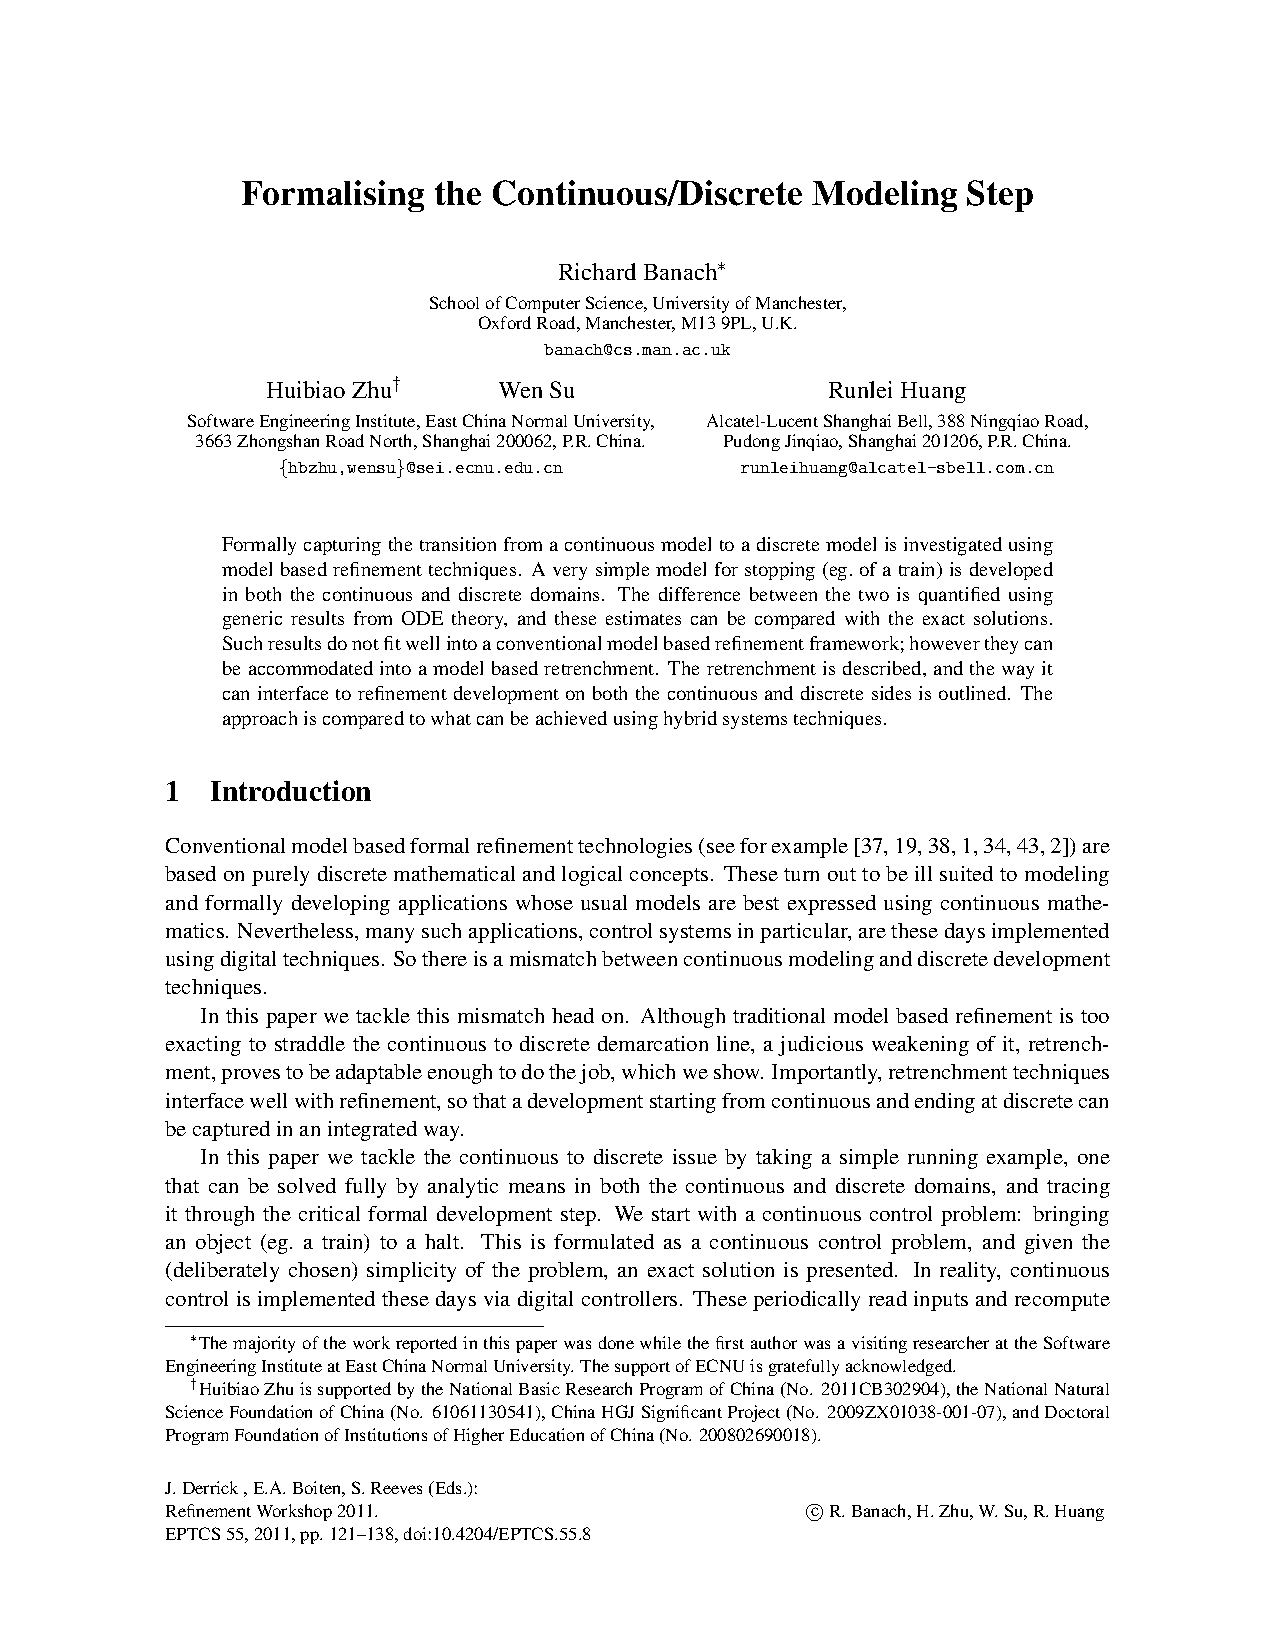
\includepdf[
  pages=-,
  trim=0 0 0 2.1cm,
  clip,
  pagecommand={\thispagestyle{fancy}}
]{foreign-original-arxiv-1106-4097v1.pdf}

\newpage
\thispagestyle{fancy}

{\centering\zihao{3}\heiti 连续/离散建模步骤的形式化\par}
\vspace{\baselineskip}
{\centering\zihao{-4}\songti Richard Banach，朱惠彪，苏文，Runlei Huang\par}
\vspace{\baselineskip}

{\zihao{-4}\songti\setstretch{1.5}\setlength{\parindent}{2em}

\noindent\textbf{摘要}

\indent 本文使用基于模型的精化技术，研究如何以形式化方式刻画从连续模型到离散模型的转换。文章分别在连续域和离散域中构造了一个非常简单的停车模型，例如列车制动模型。两者之间的差异借助常微分方程理论中的一般性结果进行量化，并且这些估计可以与精确解进行比较。这样的结果并不能很好地纳入传统的基于模型的精化框架；不过，它们可以被容纳进基于模型的弱化精化（retrenchment）之中。本文描述了这种弱化精化，并概述了它如何与连续侧和离散侧的精化开发相衔接。文章还将该方法与混合系统技术能够达到的效果进行了比较。

\subsubsection*{1 引言}

\indent 传统的基于模型的形式化精化技术建立在纯离散的数学和逻辑概念之上\,[1,19,34,37,38,43]。对于那些通常更适合用连续数学来表达的应用而言，这些技术在建模和形式化开发方面显得并不合适。然而，许多这样的应用，特别是控制系统，如今又确实通过数字技术来实现。因此，连续建模与离散开发技术之间产生了不匹配。

\indent 本文直接处理这种不匹配。传统的基于模型的精化对连续与离散之间的分界要求过于严格，难以跨越这一分界；而一种经过审慎弱化的精化形式，即弱化精化，则具有足够的适应性来完成这一任务\,[7--10,36]。更重要的是，弱化精化技术能够很好地与精化结合起来，因此从连续模型开始、最终到达离散实现的开发过程，可以用一种统一的方式来刻画。

\indent 本文通过一个简单的运行示例来处理连续到离散的问题。这个示例在连续域和离散域中都可以完全解析求解，因此可以清楚地追踪关键的形式化开发步骤。文章首先提出一个连续控制问题：使一个物体，例如一列火车，停下来。该问题被表述为连续控制问题，并且由于问题被有意设计得非常简单，文中给出了精确解。现实中，连续控制如今通常通过数字控制器实现。数字控制器会以采样周期为间隔读取输入，并在系统动态演化过程中周期性地重新计算输出。在这个意义上，控制被离散化了，尽管离散化后的控制仍然作用在连续的现实世界中。

\indent 因此，本文将连续问题重新建模为离散控制问题，并借助适当的弱化精化，对离散化步骤给出形式化描述。其论证基础来自常微分方程理论中的严格结果。受篇幅限制，本文的技术重点放在这一关键步骤上；开发过程的其余部分，即连续侧和离散侧相关精化的衔接，仅作概要说明。更完整的处理将在扩展版本中给出。

\indent 文章结构如下。第 2 节描述混合系统领域中的相关工作，并说明它们与本文方法的区别。第 3 节将列车停车问题表述为传统的开环连续控制问题。第 4 节使用简单的零阶保持策略描述控制问题的离散化。第 5 节回顾本文所需的 ASM 精化和弱化精化。第 6 节说明如何利用合适的弱化精化刻画前述离散化过程，并引用所需的常微分方程结果。第 7 节概述这些内容如何嵌入更广泛的形式化开发策略中，其中弱化精化的灵活性可以通过 Tower Pattern 与精化提供的更强保证结合。第 8 节给出结论。

\subsubsection*{2 相关工作}

\indent 连续与离散转移系统之间的关系，一直是混合系统领域的重要研究主题。较早的工作包括 Alur 等、Henzinger、Alur 与 Dill 以及 He 的研究\,[4,5,26,27]；此外，Hybrid Systems: Computation and Control 国际会议也长期汇聚了大量相关研究。较新的综述性参考可见 Tabuada 的工作\,[42]。

\indent 混合系统是将平滑的连续转移与离散的不连续转移结合起来的动态系统。该领域的主要关注点是对此类系统性质进行自动验证。显然，这种验证要求以离散且有限的方式表示相关系统：或者显式构造一个有限状态空间并直接操作，或者通过符号方式表示一个更难处理的底层状态空间，并对符号状态空间进行操作。

\indent 将难以处理的状态空间纳入可计算技术范围的主要工具是等价关系。状态空间中的区域被聚集为等价类，而这些等价类的表示，无论是简单方法中的单个元素，还是表示相应等价类的符号表达式，构成了抽象系统的状态空间。随后引入这些抽象状态之间的转移，以反映底层系统的行为。感兴趣的性质便可以在抽象系统上检查。例如，可达性性质可以落入应用于抽象系统的模型检测方法范围。

\indent 由此构造出的实际上是模拟或双模拟关系，混合系统研究的一个重要方向正是对此类模拟或双模拟进行研究。当系统受到外部控制时，同样的说明也适用。

\indent 上述方法的一个缺点是经常依赖被研究系统的脆弱性质。简单地说，许多技术依赖问题参数落在参数空间中测度为零的子集内。真实系统不可能可靠地命中这样狭小的目标。同样，所研究的模拟关系也可能同样脆弱。为了缓解这一问题并处理其他感兴趣的问题，近年来出现了近似模拟和近似双模拟的概念。这里，抽象状态 $u$ 与具体状态 $v$ 之间的模拟关系 $R(u,v)$ 不再被定义为状态上的简单谓词，而是通过距离函数 $\mathbf{d}$ 定义为
\[
R_{\epsilon}(u,v) \equiv \mathbf{d}(f(u),v) \leq \epsilon ,
\]
其中 $f$ 是两个状态空间之间在某种意义上语义自然的精确关系。对于双模拟，还需要对称安排。

\indent 模拟或双模拟依赖这样一种思想：在两个前置状态之间假定适当关系，并在合适的转移对之后的后置状态中重新建立该关系。为了保持基于距离的关系，系统动态本身需要具有稳定性。因此，关注的自然中心是稳定控制系统，通常是便于计算处理的线性稳定控制系统\,[3,6,11,18,20,22,32,40]。

\indent 在稳定系统中，所有轨迹都收敛到同一点，因此两条轨迹之间的距离单调减小；这样，基于轨迹距离的模拟关系就能被维持。不过，尽管多数系统都是按这种稳定意义来设计的，也存在一些系统或相空间区域，其轨迹会发散而不是收敛，但这并不会使系统失去用途。下文将详细处理一个非常简单的例子；在上述意义下，它恰好是不稳定的。之所以能够知道它不稳定，是因为本文可以精确求解该例子。

\indent 此外，在通常的混合系统文献中，给定系统的离散近似通常是从该系统自身制造出来的，例如通过构造等价类。相比之下，本文对离散化采取更接近工程实践的现成方式：分析连续系统的一个直接的零阶保持版本。在这种策略中，送往执行器的新输出值以固定间隔重新计算，并在下一个时间间隔内保持不变。这里的“零阶”指在整个间隔中保持输出值为常数，而不是使用更高阶保持中经过设计的高阶多项式。

\indent 因此，本文方法更接近传统工程实践，因为它关注典型的实际处理方式。当然，这两种做法并不互斥：零阶保持的参数可能落在通过原系统分析提取出的离散近似参数范围内，反之亦然。最后，本文采用弱化精化，这带来的一个结果是，分析并不限于纯稳定情形。实际上，弱化精化更强的表达能力允许类似前述模拟关系的东西既可以增大允许误差，也可以减小允许误差，尽管这一点是间接体现出来的。

\subsubsection*{3 列车停车：连续控制系统}

\indent 本文的目标应用领域是铁路中的控制问题，具体案例是列车停车。当然，在现实中，列车位置控制是一个复杂问题，需要许多机制协同工作才能获得可靠结果。本文没有篇幅处理所有这些方面及其微妙交互，而是以非常简单的方式聚焦于一个单一技术问题：连续控制问题与其离散对应物之间的关系。

\indent 假设一列质量为 $M$ 的列车以巡航速度 $V$ 行驶，现在需要停车。本文假定采用线性增加的减速度率 $a$ 是合适的。这里所谓“合适”并不是通常意义上的舒适性或可用性，而是出于简化问题的优先考虑。恒定减速度本来更简单，但恒定减速度的零阶保持近似与其自身相同，会使问题变得平凡。根据牛顿定律，为了使用线性增加的减速度使列车停下，需要施加力 $F=-Mat$，其中 $t$ 为时间。本文假设 $M$ 已知，因此只关注运动学方面。

\indent 基本运动学知识足以说明，在线性减速度下，减速度、距离和停车时间相互关联。假定存在一次停车过程，从时刻 $0$、位置 $x=0$ 开始，到时刻 $T_{Stop}$ 结束，此时列车到达位置 $x=D$。用点号表示时间导数，若 $v$ 表示速度，则有
\[
\dot{v}=-at,\qquad v(0)=V,\qquad v(T_{Stop})=0 .
\]
对于行驶距离 $x$，有
\[
\dot{x}=v,\qquad x(0)=0,\qquad x(T_{Stop})=D .
\]
积分可得
\[
V=\frac{1}{2}aT_{Stop}^{2},\qquad
D=VT_{Stop}-\frac{1}{3!}aT_{Stop}^{3}
=\frac{2}{3}VT_{Stop}.
\]

\indent 接下来将上述内容重新表述为控制理论问题。在入门层面，控制理论通常在频域中展开，因为频域中的设计技术相对简单且清晰\,[18,20,22,32]。然而，为了获得能够与形式化技术衔接的足够严格的结果，需要转向数学上更精确处理所偏好的状态空间表述\,[3,14,15,40]。在状态空间图景中，系统由若干状态变量构成，其演化由相应数量的一阶微分方程支配。状态变量和微分方程与基于模型的精化形式化中的状态和转移系统足够相似，因此有望建立联系。

\indent 对本文示例而言，为了使用一阶框架，状态必须同时包含位置 $x(t)$ 和速度 $v(t)$。因此得到状态向量
\[
\mathbf{x}(t)=
\begin{bmatrix}
x(t)\\
v(t)
\end{bmatrix}.
\]
系统动态由下式刻画：
\[
\dot{\mathbf{x}}(t)=
\begin{bmatrix}
\dot{x}(t)\\
\dot{v}(t)
\end{bmatrix}
=\mathbf{f}(\dot{x}(t),u(t))
=
\begin{bmatrix}
v(t)\\
u(t)
\end{bmatrix},
\]
其中
\[
u(t)=-at
\]
是外部控制信号。初始条件为
\[
\mathbf{x}(0)=
\begin{bmatrix}
0\\
V
\end{bmatrix}.
\]

\subsubsection*{4 从连续控制到离散控制}

\indent 要真正实现连续控制模型，需要模拟装置。在当今高度数字化的世界中，几乎不再构建这样的系统。相反，连续控制设计会被离散化，实际实现的是相应的数字控制系统。

\indent 数字控制方法与连续情形有许多相似之处。在频域中，主要区别是使用 $z$ 变换而不是拉普拉斯变换。在基于状态的图景中也有许多相似之处，只是一阶差分方程取代了一阶微分方程\,[23,24,28,33]。

\indent 本节考察上一节连续控制问题的一个离散对应物，为下一节的形式化重新评估做准备。本文示例极其简单的一个优点是，它在连续域和离散域中都允许解析解，因此后文可以对形式化重新评估作出清晰评价。

\indent 问题的出发点与前面相同：列车以速度 $V$ 行驶，需要在时间 $T_{Stop}$ 后停下，并行驶距离 $D_D$。这里下标 $D$ 用来表示离散化模型中与连续对应量不同的量。不同的是，列车并非连续地完成停车，而是在若干离散阶段中完成。令 $T_{Stop}$ 被划分为 $N$ 个短周期，每个周期长度为 $T$，于是
\[
T_{Stop}=NT .
\]

\indent 离散化方案基于零阶保持，即在单个时间周期内保持同一个控制输入值。连续处理中线性减速度率 $a$ 的对应物，是一个分段常数减速度；每经过一个长度为 $T$ 的时间间隔，常数减速度就额外减少 $a_D$ 的一个倍数。

\indent 设离散化后的速度变量为 $v_D$，加速度满足
\[
\dot{v}_D(t)=-ka_DT,
\]
其中
\[
k=\left\lceil \frac{t}{T}\right\rceil,
\]
且 $k$ 的取值范围为 $1,\ldots,N$。对于一般的 $t$，令
\[
\delta t_k=t-(k-1)T=t-\left\lfloor \frac{t}{T}\right\rfloor T .
\]
考虑初始速度为 $V$，当 $(k-1)T<t<kT$ 时，第 $k$ 个周期内速度为
\[
v_D(t)=V-a_DT^2-2a_DT^2-\cdots-(k-1)a_DT^2-ka_DT\delta t_k .
\]
由于最终速度为零，得到
\[
V=a_DT^2+2a_DT^2+\cdots+Na_DT^2
=\frac{1}{2}a_DT^2N(N+1).
\]

\indent 已知速度后，再次积分可求得行驶距离。令离散世界中的位移为 $x_D$，在区间 $(k-1)T<t<kT$ 中对 $x_D$ 的贡献为
\[
\left(V-a_DT^2-2a_DT^2-\cdots-(k-1)a_DT^2\right)\delta t_k
-\frac{1}{2}ka_DT\delta t_k^2 .
\]
因此总距离为
\[
D_D=NV T
-a_DT^3\sum_{k=1}^{N-1}(N-k)k
-\frac{1}{2}a_DT^3\sum_{k=1}^{N}k ,
\]
也即
\[
D_D=VT_{Stop}
-\frac{1}{12}a_DT^3(2N^3+3N^2+N).
\]
将 $a_D$ 的值代入可得
\[
D_D
=VT_{Stop}\left[1-\frac{2N^2+3N+1}{6N^2+6N}\right]
=\frac{2}{3}VT_{Stop}\left[1-\frac{1}{4N}+O(N^{-2})\right].
\]

\indent 可以看到，在保持 $V$ 与 $T_{Stop}$ 相同的情况下，$D_D$ 相对于连续情形中的 $D$ 包含一个 $O(1/N)$ 修正。这是因为要求 $T_{Stop}$ 必须是 $T$ 的整数倍，产生了额外约束；如果还希望 $D$ 与 $D_D$ 完全相同，问题就会被过度约束。

\indent 按照前一节的一阶初值系统形式重写并不困难。状态向量为
\[
\mathbf{x}_D(t)=
\begin{bmatrix}
x_D(t)\\
v_D(t)
\end{bmatrix},
\]
系统动态为
\[
\dot{\mathbf{x}}_D(t)=
\begin{bmatrix}
\dot{x}_D(t)\\
\dot{v}_D(t)
\end{bmatrix}
=\mathbf{f}(\dot{x}_D(t),u_D(t))
=
\begin{bmatrix}
v_D(t)\\
u_D(t)
\end{bmatrix},
\]
其中
\[
u_D(t)=\dot{v}_D(t)=-ka_DT
\]
是外部控制。初始条件为
\[
\mathbf{x}_D(0)=
\begin{bmatrix}
0\\
V
\end{bmatrix}.
\]

\indent 与连续模型相比，上述离散模型明显复杂得多。离散系统通常都是如此，这也是人们强烈希望在连续域中建模系统的原因。连续问题离散化后复杂性迅速上升，正是本文选择特别简单示例的理由。在这样的研究中，使复杂性仍然足够低以允许精确求解非常有用，因为这使得精确方法和近似方法之间的比较可以更有把握地进行。

\subsubsection*{5 ASM 精化与弱化精化}

\indent 本节回顾本文所需的 ASM 精化和弱化精化，它们是本文形式化工作的载体。ASM 方法的标准参考建立在早期 ASM 精化工作的基础上\,[12,13]。一般而言，为了证明一个 ASM 精化，需要验证所谓的 $(m,n)$ 图。在这种图中，$m$ 个抽象步骤模拟 $n$ 个具体步骤。本文只需关注体现这一策略的精化证明义务。

\indent 第一个证明义务是初始化证明义务：
\[
\forall y'\bullet CInit(y')\Rightarrow
(\exists x'\bullet AInit(x')\land R(x',y')) .
\]
这要求对于每一个具体初始状态 $y'$，都存在一个抽象初始状态 $x'$，使得检索关系或抽象关系 $R(x',y')$ 成立。

\indent 第二个证明义务是正确性，涉及对 $(m,n)$ 图的验证。假设已经决定哪些 $(m,n)$ 图足以覆盖应用所需情形。令 $CFrags$ 表示那些具体执行片段的集合，它们能够覆盖应用中所有感兴趣的具体执行序列。记 $y::ys::y'\in CFrags$ 表示以具体状态 $y$ 开始、以具体状态 $y'$ 结束、中间状态序列为 $ys$ 的片段。类似地，$x::xs::x'\in AFrags$ 表示抽象片段。令 $is,js,os,ps$ 分别表示属于抽象片段和具体片段的抽象输入、具体输入、抽象输出、具体输出序列，并用 $In(is,js)$ 与 $Out(os,ps)$ 表示合适的输入和输出关系。

\indent 正确性证明义务要求：若存在一个由具体操作序列执行的具体执行片段，并且具体与抽象的前置状态以及输入之间满足检索关系和输入关系，则必须能找到一个抽象执行片段，使其重新建立检索关系和输出关系。ASM 精化策略还要求从具体到抽象保持非终止性，但本文不需要这一点。

\indent 弱化精化也由证明义务刻画\,[7--10,36]。其初始化证明义务与上述精化的初始化证明义务相同；而“正确性”证明义务则通过在精化正确性证明义务中插入 \textit{within}、\textit{output} 和 \textit{concedes} 关系而得到弱化，分别记为 $W_{Op}$、$O_{Op}$ 和 $C_{Op}$。其中，让步关系 $C_{Op}$ 以析取方式弱化结论，为许多种“异常”行为留出表达空间。

\indent 为了保证弱化精化只处理定义良好的转移，并使弱化精化与精化能够平滑协作，还要求 $R\land W_{Op}$ 总是落在所需操作的定义域内，尽管本文同样不需要使用这一点。

\indent 精化与弱化精化之间的平滑协作由 Tower Pattern 保证。在该基本构造中，精化为纵向箭头，弱化精化为横向箭头。从模型 $A$ 到模型 $D$ 绕方形的两条路径是相容的：一条先组合 $A$ 到 $C$ 的精化再组合 $C$ 到 $D$ 的弱化精化，另一条先组合 $A$ 到 $B$ 的弱化精化再组合 $B$ 到 $D$ 的精化。两者都定义了从 $A$ 到 $D$ 的某个潜在更大弱化精化的一部分。

\indent 这一点与本文案例的联系在于：虽然本文考虑的动态完全处在连续域中，但 ASM 证明义务关注的是抽象层和具体层上的路径。基于这种路径视角，可以将 $(m,n)$ 规则重新配置为处理连续路径而不是离散跳转。因此，$CFrags$ 和 $AFrags$ 可以指连续系统轨迹片段，而不是状态到状态的跳跃序列；$W$ 中的输入序列也可以指轨迹上的连续输入信号。第 6 节将详细展示这种思想。

\subsubsection*{6 连续到离散建模变化的形式化}

\indent 在控制文献中，可以找到许多离散化连续设计的方法，而对连续与离散关系的评估通常基于工程中的经验规则。虽然这些规则在实践中通常能产生完全可用的结果，但其判据远未达到与基于模型的形式化开发技术良好衔接所需的精确程度。因此，当基于模型的形式化开发技术用于支持某个连续设计之离散对应物的数字实现时，形式化建模通常不可避免地已经从离散域开始。显然，与从连续设计阶段更早开始并贯穿后续所有设计步骤的形式化建模相比，这对开发过程提供的形式化支持较弱。

\indent 本文的目标是说明如何对控制问题的离散化作出足够精确的判断，使其能够与基于模型的形式化技术良好集成。为此，本文诉诸常微分方程的严格理论。可以证明，仅在输入控制上不同的两个控制问题实例满足不等式\,[3,14,15,40]
\[
\|\mathbf{x}^{u}-\mathbf{x}_{D}^{u_D}\|\leq K2\|u-u_D\|_2 .
\]
其中，$\|\mathbf{x}^{u}-\mathbf{x}_{D}^{u_D}\|$ 是 $\mathbf{x}^{u}-\mathbf{x}_{D}^{u_D}$ 的 $\mathcal{L}^{\infty}$ 范数，通俗地说，就是在区间 $[0,\ldots,T_{Stop}]$ 上连续状态和离散状态任一分量差值所能达到的最大值。$\|u-u_D\|_2$ 是 $u-u_D$ 的 $\mathcal{L}^{2}$ 范数，通俗地说，是在同一区间上计算得到的输入差值平方积分的平方根。$K2$ 是一个常数。

\indent 本文案例中的连续版本和离散版本，具有相同形式的初始状态，并且都在 $0$ 到 $T_{Stop}$ 的时间区间上演化。它们恰好刻画了这种场景，因为连续模型与离散模型只是在独立变量中使用 $u_D$ 而不是 $u$。

\paragraph{6.1 连续系统与离散系统的严格界}

\indent 现在说明上述不等式对本文小案例意味着什么。为了得到左侧差异的界，需要考察右侧各量的取值。理论给出了常数 $K2$ 的显式值：
\[
K2=e^{K_{\mathbf{f}}}\|k_u\|_2 .
\]
其中，$K_f$ 为 $k_fT_{Stop}$，$k_f$ 是 $\mathbf{f}_{\mathbf{x}}$ 的 $\mathcal{L}^{\infty}$ 范数，即在区间 $[0,\ldots,T_{Stop}]$ 上，控制律 $\mathbf{f}$ 关于状态变化的 Lipschitz 常数的绝对最大值。本文应用中的控制律形式为
\[
\mathbf{f}(v(t),u(t))=
\begin{bmatrix}
v(t)\\
u(t)
\end{bmatrix}.
\]
显然，$\mathbf{f}$ 中只有一个分量关于 $x$ 或 $v$ 的偏导数非零，即
\[
\frac{\partial \mathbf{f}_1}{\partial v}=1 .
\]
因此第一个因子为 $e^{T_{Stop}}$。

\indent 第二个因子 $\|k_u\|_2$ 是控制律关于输入控制信号变化的 Lipschitz 常数的平方积分平方根。同样，$\mathbf{f}$ 中只有第二个分量关于 $u$ 的偏导数非零：
\[
\frac{\partial \mathbf{f}_2}{\partial u}=1 .
\]
所以平方积分平方根化为 $\sqrt{T_{Stop}}$，得到
\[
K2=e^{T_{Stop}}\sqrt{T_{Stop}} .
\]

\indent 接下来考虑 $\|u-u_D\|_2$。根据前面的计算，
\[
u(t)=-at,\qquad u_D(t)=-ka_DT,
\]
且
\[
a=\frac{2V}{T_{Stop}^{2}},\qquad
a_D=\frac{2V}{T_{Stop}^{2}(1+1/N)} .
\]
由此可见，$u(t)$ 线性下降，而 $u_D(t)$ 是一条在 $u(t)$ 附近按等距台阶下降的阶梯函数。当 $t\to 0+$ 时，$u(0+)=0$，而 $u_D(0+)=-a_DT$，因此 $u(0+)-u_D(0+)=a_DT$。当 $t\to T_{Stop}-$ 时，$u(T_{Stop}-)=-aT_{Stop}$，而 $u_D(T_{Stop}-)=-Na_DT=-a_DT_{Stop}$，于是二者差为 $-a_DT$。由于阶梯具有等间距步长，$u_D(t)$ 显然在 $u(t)$ 周围以 $a_DT$ 为界变化：
\[
|u(t)-u_D(t)|\leq a_DT .
\]
因此，
\[
\|u-u_D\|_2
\leq
\sqrt{\int_{0}^{T_{Stop}}(a_DT)^2dt}
=a_DT\sqrt{T_{Stop}} .
\]
代入前述不等式，得到
\[
\|\mathbf{x}^{u}-\mathbf{x}_{D}^{u_D}\|
\leq
e^{T_{Stop}}\sqrt{T_{Stop}}\cdot a_DT\sqrt{T_{Stop}}
=e^{T_{Stop}}a_DTT_{Stop}.
\]

\indent 可以看到，虽然 $u(t)$ 与 $u_D(t)$ 之间的偏差可能随着时间区间长度以指数方式增长，而且本文使用的界较为粗略而加剧了这种可能性，但总可以通过使离散化足够细，即增大 $N$，将偏差任意减小。

\paragraph{6.2 将严格界转化为弱化精化数据}

\indent 现在已经获得连续控制系统与离散控制系统之间的精确关系，可以将其纳入基于模型的形式化描述。一般而言，基于模型的形式化精化要求过于严格，无法容纳刚刚推导出的关系；弱化精化正是为此类情形而设计的，因此本文采用弱化精化。

\indent 无论采用哪种基于模型的形式化描述技术，都存在一个问题：这些技术通常面向离散状态转移，并假定存在定义良好的“下一状态”概念，以便与同样清楚的“当前状态”概念相关联。在连续动态中，并不存在一个可以直接使用的合理“下一状态”概念。不过，如前所述，ASM 精化中的 $(m,n)$ 图方法表明，被关联的是抽象层和具体层上的路径。因此，本文扩展 ASM 方法，使其既可包含连续路径，也可包含离散路径。这也是本文选择 ASM 的一个重要原因。

\indent 在连续问题中，存在一条连续路径；在离散化问题中，则存在 $N$ 条连续的较短“零阶保持”路径，它们在时刻 $kT$ 处与输出信号的离散重新计算交错，从而形成一条同时包含连续和离散成分的路径。由于本文使用的严格结果要求两个系统从同一初始状态出发，因此形式化陈述被约束为端到端关系。它表达了连续层平滑动态与离散层动态之间的端到端关系；后者同样是连续的，只是每个 $T$ 的整数倍时刻都会发生加速度的不连续变化。

\indent 一个弱化精化由四部分组成：状态空间之间的检索关系、前置状态和输入的 within 关系、后置状态和输出的 output 关系，以及后置状态和输出的 concedes 关系。对于检索关系 $R$，最自然的选择似乎是连续世界与离散化世界中状态值之间的恒等关系。然而，尽管本文具体案例中两个模型确实从同一状态开始，但在多数情形下这一假设并不成立，因此作者选择更通用的方式。另一种选择是让 $R$ 表示连续和离散状态值之间的容差范围，这类似相关工作中讨论的近似模拟关系。不过，当两个系统状态之间的关系在整个动态过程中稳定时，这种方案最有效；而本文案例中该假设不成立，因为两个系统状态之间的差异会随动态过程持续增长。

\indent 为了处理这种不便利的情况，弱化精化允许在 within 关系 $W$ 中表达转移前置点处状态之间的关系或其某些方面，而不是在 $R$ 中表达。由于 $W$ 中表达的事实不需要在证明义务结论中重新建立，这为把系统前置状态中的适当事实纳入证明义务提供了最灵活的方式。基于这一策略，本文将全局检索关系设为真：
\[
R(\langle x(t),v(t)\rangle,\langle x_D(t),v_D(t)\rangle)\equiv \textsf{true}.
\]

\indent 表达前置状态适当匹配的任务由 within 关系 $W$ 承担，同时还要考虑整个目标区间内的输入控制信号：
\[
\begin{aligned}
W\equiv{}&x(0)=x_D(0)\land v(0)=v_D(0)\\
&\land \|u-u_D\|_2\leq a_DT\sqrt{T_{Stop}} .
\end{aligned}
\]
注意，$W$ 不仅关联连续和离散的前置状态，还关联整个连续和离散控制输入。

\indent output 关系 $O$ 描述目标时间段结束时发生了什么。根据前面的计算，可以使用 $O$ 说明两个系统的后置状态差异不超过已经推导出的界：
\[
\begin{aligned}
O\equiv{}&|x(T_{Stop})-x_D(T_{Stop})|
\leq e^{T_{Stop}}a_DTT_{Stop}\\
&\land |v(T_{Stop})-v_D(T_{Stop})|
\leq e^{T_{Stop}}a_DTT_{Stop}.
\end{aligned}
\]
虽然 $O$ 本身显式谈论的是两个系统到达的后置状态，但这些性质是通过 $\mathcal{L}^{\infty}$ 分析推导出来的，因此同样的界实际上在整个目标区间内都成立。这种表述的优点是，描述自动呈现为前置状态和后置状态之间的离散形式，能够与离散系统推理器良好集成，同时仍然提供贯穿整个时间区间的保证。

\indent 由于本文系统非常简单，$O$ 已经捕获了所有需要表达的内容，在更真实工程情形中可能需要考虑的异常行为并不存在。这也与本文将检索关系平凡化有关。因此，可以将 concedes 关系 $C$ 设为假：
\[
C(\langle x(T_{Stop}),v(T_{Stop})\rangle,
\langle x_D(T_{Stop}),v_D(T_{Stop})\rangle)\equiv \textsf{false}.
\]
有了这些数据，弱化精化证明义务可基于前述结果得到证明，从而建立连续域与离散域之间的形式化联系，并且这种联系可以与连续侧和离散侧的形式化精化集成。

\indent 特别值得注意的是，状态之间的差异随时间线性增长；这是精确解的性质，并非某种近似方案的假象。如果试图在纯精化框架中处理这一点，用检索关系 $R$ 捕捉两个模型状态之间的关系，无论 $R$ 是精确逐点关系还是类似近似模拟关系的近似关系，都无法从前置状态中假定的 $R$ 在后置状态中重新建立它，因此正确性证明义务不能被证明。弱化精化的更大灵活性允许在 within 关系中处理前置状态，在 output 关系中处理后置状态，从而克服这一问题。

\paragraph{6.3 验证性佐证}

\indent 在本文案例中，连续和离散控制模型均可精确求解，这为本文倡导的方法提供了额外且独立的确认。两个模型运行相同的时间 $T_{Stop}$，output 关系给出了该时间后两个模型到达状态之间差异的估计。状态由位移和速度两个分量构成。

\indent 关于速度，两个模型在 $T_{Stop}$ 后都完全停止。因此 $v(T_{Stop})$ 与 $v_D(T_{Stop})$ 都为零，二者差值为零，任何正上界都是可靠的。因此，前述 output 关系给出的速度差上界是正确的，但并不令人惊讶。

\indent 关于位移，离散情形中 $T_{Stop}$ 的量化使连续动态和离散动态停在略微不同的位置，即 $D$ 和 $D_D$。基于前面的计算，可以得到精确差值：
\[
|x(T_{Stop})-x_D(T_{Stop})|
=\frac{1}{12}a_DT T_{Stop}^{2}\left(1+\frac{1}{N}\right).
\]
另一方面，output 关系给出的估计为
\[
e^{T_{Stop}}a_DTT_{Stop}.
\]
因此，精确值落在估计界内，当且仅当消去公共因子 $a_DTT_{Stop}$ 后满足
\[
\frac{T_{Stop}}{12}\left(1+\frac{1}{N}\right)\leq e^{T_{Stop}} .
\]
斜率小于 $1$ 的 $T_{Stop}$ 线性函数不可能追上系数为 $1$ 的指数函数，因此该不等式显然成立，验证性佐证由此得到。

\subsubsection*{7 更广泛设计过程中的连续到离散建模}

\indent 前几节详细关注常微分方程的严格理论如何在一个非常简单的例子中产生能够与现有基于模型的精化中心开发方法集成的结果。该过程的核心是从数学理论中识别有用结果，然后深入证明细节以识别其中出现的常数等量的显式值。后一过程经常是必要的，因为感兴趣证明的目标通常只需断言所需常数存在，而不必计算具体值；这足以证明某种极限存在。相比之下，对工程过程而言，极限的存在是不够的，因为任何工程过程都不可能完整走完到达极限所需的无限道路。本文需要所有量的显式值，以便判断需要沿这条道路走多远，才能确信已经足够达到所需的工程质量。

\indent 本节概述以这种方式获得的弱化精化如何置于更广范围的开发方法中。由于篇幅限制，若干技术问题只能简要涉及。集成的关键思想是前文提到的 Tower Pattern。它允许将弱化精化的极端灵活性，即容纳多种系统性质的能力，与基于模型的精化提供的严格得多的保证相结合。后者以系统性质表达能力受到更多限制为代价。作者认为，两种技术的审慎结合，比任何单独技术都能更好地覆盖从高层领域需求目标到低层实现的路径。

\indent 一方面，仅使用精化会迫使开发者过早考虑并承诺低层限制，例如算术的有限性界限，以便所有后续模型在实质上都成为其前驱模型的保守扩展。另一方面，仅使用弱化精化又会使跟踪系统性质随开发推进而如何演化变得困难，因为连续模型可能以非常松散的方式与前驱模型相连，从而需要更加关注事后验证。

\indent 在本文情形中，用弱化精化捕获离散化步骤的性质是合适的，因为该步骤一直难以被基于模型的精化技术处理。需要指出的是，近似模拟的引入近年已经改善了稳定系统相关情形，但在更一般语境中，上述观察仍然成立。不过，在离散化步骤两侧，可以自由使用精化，因为在每一侧内部，模型在可用精化充分表达的性质类型方面具有更强的一致性。

\indent 文章用整体开发图概括了作者设想的完整过程。图中的粗箭头追踪一族模型中一条可能的开发路线。图左侧涉及连续模型。起点是高层需求目标，用具有形式基础的记法表达；作者想到的是类似 KAOS 的形式主义，或者更准确地说，是一种能够更诚实处理连续过程的 KAOS 适配形式\,[30,31]。这些需求目标可以被形式化精化，直到它们能够被操作化，也就是转化为 ASM 等方法的操作。随后进入离散化步骤，此时需要使用弱化精化。一旦跨过连续/离散边界，就可以回到传统的基于模型的离散状态转移系统精化技术，不再担心连续现象。

\indent 图中还展示了离散运动学如何进一步精化为列车制动模型，在后者中，对动态的关注被执行器层面的关注所取代，这些执行器在实践中实现减速度增量。图中还用星号表示其他模型；这些模型的存在由 Tower 定理保证，使图中的方形以适当意义交换。不过，作者认为这些模型没有其他模型实用。例如，左下角模型将是制动模型的连续版本，在如此接近实现的位置上显得不现实且过度理想化。右上角模型将是最高层列车停车需求目标的离散化版本，这在如此高的抽象层次上同样不合适，因为它会把大量关于离散化方案低层细节的材料加入本应最清晰表达系统目标的模型中。

\indent 文中还简要讨论了 KAOS 和 ASM 对连续行为的适配。对于 ASM，所需内容已有相当一部分存在于文献中，例如 Real Timed ASM\,[16,39]。基本观察是：在连续时间语境下，系统状态应被建模为在半开半闭时间区间上持续存在，例如 $(t_0,t_1]$。这使得典型离散转移系统中某个状态变量 $v$ 的不连续状态转移，可以表示为从 $v(t_0)$ 转向 $\lim_{\epsilon\to0+}v(t_0+\epsilon)$。同样，一段连续演化可理解为在这样的半闭区间上持续，由适当良定的常微分方程初值问题支配，并以前一时间区间末端初值条件成立作为系统随后沿常微分方程指定轨迹演化的触发条件。采用这些约定，可以发展出一种离散步骤与连续流交替出现的 ASM 版本，反映混合自动机的许多特征。

\indent KAOS 也可采用类似方法。虽然 KAOS 从一开始就依赖时间概念，但通常的 KAOS 形式主义中时间是离散的，一般由整数索引，需求目标用关于时间的时序逻辑公式表达。在连续时间版本中，某些时序算子，例如“总是”和“直到”，没有概念困难；但“下一步”算子需要重新考虑。仍然可以使用半开半闭区间，并通过半闭区间左端点处的右极限来定义后继状态。为了避免多个“下一步”算子累积造成的问题，需要对允许的时序公式施加句法限制。不过，KAOS 需求通常所基于的模式满足这些限制。

\subsubsection*{8 结论}

\indent 本文以状态空间格式引入了一个小型连续控制问题，并使用零阶保持处理了它的离散化对应物。随后，文章给出了主要的新贡献：基于常微分方程理论中的已有结果，对连续到离散建模转换进行严格处理。完成这一点后，作者能够将结果集成到一个弱化精化中，用来关联连续模型和离散模型。正如前文指出的，基于模型的形式化开发通常已经从离散域开始，因此能够以有根据的方式将其与连续世界连接起来，显著扩展了基于模型的形式化技术支撑此类系统开发的潜力。同样重要的是，本文本质性地使用弱化精化来建立连续建模和离散建模之间的联系，这进一步确认了弱化精化作为精化补充概念在处理现实世界形式化开发更广泛问题时的价值。

\indent 当然，本文远不是此类开发的最终结论。本文处理的控制问题在技术上几乎是平凡的，并且使用的数学控制理论严格结果也相对有限：它要求被比较的两个行为从同一状态开始，使用对控制输入差异较粗略的 $\mathcal{L}^{2}$ 估计来推出结论，并建立在支配控制问题动态的常微分方程的一般性质之上。这些简单约束也意味着本案例只使用了弱化精化表达能力中相对较小的一部分。

\indent 在更真实的情形中，问题通常不太可能解析求解，反馈机制将有助于缓解固有不确定性。此外，粗略的 $\mathcal{L}^{2}$ 输入差异估计允许两个控制输入之间的距离达到控制空间界限所允许的程度；而实践中，反馈机制往往会推动它们靠近，这可以被利用来推导连续和离散控制之间差异的更严格估计。所有这些都留待未来工作讨论，对 KAOS 和 ASM 形式主义进行扩展，使其能够涵盖本文所描述的连续行为，也同样属于未来工作。

\indent 本文工作需要与混合系统方法的可能性相对照。在混合系统方法中，坚持连续系统与离散对应物之间的近似双模拟，会将关注限制在 Liapunov 意义下稳定的控制系统上。无论如何，该领域强烈关注算法可判定性，并以自动机同态作为系统模型之间的重要关系，这可能抑制本文所关心的设计表达能力。例如，严格来说，依赖稳定性的技术并不适用于本文这个简单案例。

\indent 一旦建立起一组适用范围广且有用的此类结果，就可以将它们纳入适当的形式化开发工具。这些工具的风格会不同于混合系统领域通常开发的工具，因为它们会更强调交互式证明。需要克服的一个障碍是，大多数基于证明的工具并不擅长处理本文所需的应用数学和严格分析技术。一个显著例外是 PVS 工具套件，它具有大量库支持，可支撑应用数学及其更严格的对应内容\,[17,21,35]。因此，PVS 将是开发与本文方法相匹配工具的自然起点。

\subsubsection*{译文参考文献}

{\setlength{\parindent}{0em}
\setlength{\hangindent}{2em}
[1] ABRIAL J-R. The B-Book: Assigning Programs to Meanings[M]. Cambridge: Cambridge University Press, 1996.\par
[2] ABRIAL J-R. Modeling in Event-B: System and Software Engineering[M]. Cambridge: Cambridge University Press, 2010.\par
[3] AHMED N. Dynamic Systems and Control with Applications[M]. Singapore: World Scientific, 2006.\par
[4] ALUR R, COURCOUBETIS C, HENZINGER T, HO P-H. Hybrid automata: An algorithmic approach to the specification and verification of hybrid systems[C]//Proc. Workshop on Theory of Hybrid Systems. Berlin: Springer, 1993: 209--229.\par
[5] ALUR R, DILL D. A theory of timed automata[J]. Theoretical Computer Science, 1994, 126: 183--235.\par
[6] ANTSAKLIS P, MICHEL A. Linear Systems[M]. Boston: Birkhauser, 2006.\par
[7] BANACH R. Model based refinement and the design of retrenchments[EB/OL]. Available from Retrenchment Homepage.\par
[8] BANACH R, JESKE C. Retrenchment and refinement interworking: the Tower Theorems[J]. Submitted.\par
[9] BANACH R, JESKE C, POPPLETON M. Composition mechanisms for retrenchment[J]. Journal of Logic and Algebraic Programming, 2008, 75: 209--229.\par
[10] BANACH R, POPPLETON M, JESKE C, STEPNEY S. Engineering and theoretical underpinnings of retrenchment[J]. Science of Computer Programming, 2007, 67: 301--329.\par
[11] BARNETT S. Introduction to Mathematical Control Theory[M]. Oxford: Oxford University Press, 1975.\par
[12] BOERGER E. The ASM refinement method[J]. Formal Aspects of Computing, 2003, 15: 237--257.\par
[13] BOERGER E, STAERK R F. Abstract State Machines: A Method for High Level System Design and Analysis[M]. Berlin: Springer, 2003.\par
[14] CLARKE F. Optimization and Nonsmooth Analysis[M]. Philadelphia: Society for Industrial Mathematics, 1987.\par
[15] CLARKE F, LEDYAEV Y, STERN R, WOLENSKI P. Nonsmooth Analysis and Control Theory[M]. Berlin: Springer, 1997.\par
[16] COHEN J, SLISSENKO A. Implementation of Timed Abstract State Machines with Instantaneous Actions by Machines with Delays[R]. Technical Report TR-LACL-2008-2. LACL, University of Paris-12, 2008.\par
[17] CROW J, OWRE S, RUSHBY J, SHANKAR N, SRIVAS M. A tutorial introduction to PVS[C]//WIFT'95: Workshop on Industrial-Strength Formal Specification Techniques. IEEE Computer Society Press, 1995.\par
[18] D'AZZO J, HOUPIS C. Linear Control System Analysis and Design: Conventional and Modern[M]. New York: McGraw Hill, 1995.\par
[19] DERRICK J, BOITEN E. Refinement in Z and Object-Z: Foundations and Advanced Applications[M]. London: Springer-Verlag UK, 2001.\par
[20] DORF R, BISHOP R. Modern Control Systems[M]. Upper Saddle River: Pearson, 2010.\par
[21] DUTERTRE B. Elements of Mathematical Analysis in PVS[C]//TPHOLS 1996. LNCS 1125. Berlin: Springer, 1996.\par
[22] DUTTON K, THOMPSON S, BARRACLOUGH B. The Art of Control Engineering[M]. Boston: Addison Wesley, 1997.\par
[23] FADALI M, VISIOLI A. Digital Control Engineering: Analysis and Design[M]. Amsterdam: Academic Press, 2009.\par
[24] FRANKLIN G, POWELL J, WORKMAN M. Digital Control Systems[M]. Upper Saddle River: Prentice Hall, 1996.\par
[25] HE J. From CSP to hybrid systems[C]//ROSCOE A W, ed. A Classical Mind, Essays in Honour of C. A. R. Hoare. London: Prentice-Hall International, 1994: 171--189.\par
[26] HENZINGER T A. The theory of hybrid automata[C]//Proc. IEEE LICS-96. Piscataway: IEEE, 1996: 278--292.\par
[27] IEEE Standard 1474. IEEE Standard for Communications-Based Train Control (CBTC) performance, functional, user interface, system design and functional allocation requirements[S]. IEEE Std 1474.1-2004, IEEE Std 1474.2-2003, IEEE Std 1474.3-2008.\par
[28] JESKE C. Algebraic Integration of Retrenchment and Refinement[D]. Manchester: University of Manchester, 2005.\par
[29] KUO B. Digital Control Systems[M]. Oxford: Oxford University Press, 1992.\par
[30] van LAMSWEERDE A. Requirements Engineering: From System Goals to UML Models to Software Specifications[M]. Hoboken: Wiley, 2009.\par
[31] LETIER E. Reasoning about Agents in Goal-Oriented Requirements Engineering[D]. Louvain-la-Neuve: Universite Catholique de Louvain, 2001.\par
[32] OGATA K. Modern Control Engineering[M]. Upper Saddle River: Pearson, 2008.\par
[33] PARASKEVOPOULOS P. Digital Control Systems[M]. Upper Saddle River: Prentice Hall, 1996.\par
[34] POTTER B, SINCLAIR J, TILL D. An Introduction to Formal Specification and Z[M]. 2nd ed. Upper Saddle River: Prentice Hall, 1996.\par
[35] PVS Homepage[EB/OL]. http://pvs.csl.sri.com.\par
[36] Retrenchment Homepage[EB/OL]. http://www.cs.man.ac.uk/retrenchment.\par
[37] de ROEVER W P, ENGELHARDT K. Data Refinement: Model-Oriented Proof Methods and their Comparison[M]. Cambridge: Cambridge University Press, 1998.\par
[38] SEKERINSKI E, SERE K. Program Development by Refinement: Case Studies Using the B-Method[M]. Berlin: Springer, 1998.\par
[39] SLISSENKO A, VASILYEV P. Simulation of Timed Abstract State Machines with Predicate Logic Model Checking[J]. Journal of Universal Computer Science, 2008, 14: 1984--2006.\par
[40] SONTAG E. Mathematical Control Theory[M]. Berlin: Springer, 1998.\par
[41] SU W, YANG F, WU X, GOU J, ZHU H. Formal approaches to mode conversion and positioning for vehicle systems[C]//Proc. 3rd IEEE International Workshop on Security Aspects of Process and Services Engineering. To appear, 2011.\par
[42] TABUADA P. Verification and Control of Hybrid Systems: A Symbolic Approach[M]. Berlin: Springer, 2009.\par
[43] WOODCOCK J, DAVIES J. Using Z, Specification, Refinement and Proof[M]. Upper Saddle River: Prentice Hall, 1996.\par}

\par}
\endgroup

\end{document}
